\chapter{Introduction}
\pagenumbering{arabic} 
\setcounter{page}{1} 

% General biological modeling
Despite more than a century of active biology research, running biological experiments is still time consuming and difficult.
Therefore, having a good computational model of the biological system of interest is incredibly valuable.
What makes a computational model good?
Most importantly, a good model needs to accurately describe how the biological system acts in the real world.
A model is only useful if it accurately represents the biological system and can be used to help answer research questions.
This allows experiments and hypotheses to be tested using a model instead of in vivo, speeding up the pace of research.
A good model should also be consistent--meaning it should facilitate running the same experiment multiple times and getting the same results.
Though biological experiments can have wide variance due to external conditions, we want our model to vary only due to intrinsic biological sources of variation.
Exact reproducibility is very difficult in laboratory environments, but a computer model can and should eliminate the extrinsic sources of variance that one encounters in a laboratory setting.
Finally, the best models not only describe the system, but also facilitate deeper insights into the underlying biology.
A good model should help researchers improve their understanding of the system that is modeled and provide a starting point for novel insights.

%Recent efforts to model biological systems have become ever more accurate as the amount of biological data collected increases.
Biological organisms are incredibly complex systems that can be examined at many different levels.
For example, one model could use a physical description of the system to predict the shape of an cell as it grows.
A different model could use -omic data--genomic, transcriptomic, and metabolomic measurements--to model the production of compounds that allow for cellular growth.
As all models are inherently limited in some way, so the choice of what type of model that is used to describe a system is extremely important.

This dissertation will focus on using experimental data and dimensionality reduction techniques to build a metabolic model for cell-free systems.
In particular, we use a Variational Autoencoder (VAE) with a custom loss function on top of a common metabolic modeling technique called Flux Balance Analysis  (FBA).
We combine these tools to build a pipeline that learns which reactions are most important for a given cell-free system.
The goal is to provide a model for biologists to better understand what is occurring in cell-free systems.
This will allow them to anticipate how different starting conditions will affect their experiments before actually running the experiment.

\textbf{Metabolic models}
Metabolism is defined as all of the chemical reactions that occur within an entity--usually an organism or a cell--in order to sustain its life and growth.
Biologists are extremely interested in how the metabolism of a system works as it is the end result of the other biological process of interest (e.g. transcription and translation).
Ongoing work continues to develop a more robust understanding the metabolism, while recent advances have begun to customize the metabolism. 
Metabolic engineering is particularly interesting for its potential to create novel advances in medicine and energy production~\cite{keasling2012synthetic}.
One of the most important tools in aiding metabolic engineers are metabolic models.
These models are used to predict how the phenotype of the organism will respond to various environmental inputs or changes performed by the metabolic engineer.

Most metabolic models represent the chemical reactions in a cell through a mathematical representations of the reaction coefficients.
Individual reactions are represented as equations in these models.
These reactions can then be constrained based on our knowledge of biological pathways.
Models of this type are collected under the heading of constraint-based reconstruction and analysis (COBRA) models~\cite{schellenberger2011quantitative} and are very common among the metabolic engineering community~\cite{orth2010flux}.
In particular, Flux Balance Analysis (FBA), is one of the most popular metabolic modeling techniques that has been used in hundreds of different works on metabolism~\cite{feist2008growing}.
These applications range from optimizing metabolic pathways~\cite{almaas2004global} to investigating gene networks~\cite{shlomi2007genome}.
FBA is based on a genome scale metabolic models (GEMs) reconstructed from the genome of an organism of interest.
However, these GEMs describe living organisms, not cell-free systems, thus most FBA models cannot be applied out of the box to a cell-free system.

\textbf{Cell-free systems}
Cell-free protein synthesis (CFPS) systems are a reduced version of cells that allows these systems to produce proteins without being alive.
The Central Dogma of biology, as enunciated by Francis Crick, is that DNA makes RNA makes protein~\cite{crick1970central}.
While this may be a slight oversimplification, the point remains that the production of protein is the end goal for biological systems.
CFPS systems take that to an extreme by removing all endogenous DNA and RNA and membranes while retaining the machinery crucial for transcription and translation.
A CFPS system is therefore a type of programmable matter, a veritable biological computer.
The CFPS system acts like a computer because it can "execute" any DNA "program" that is added to the mixture.
The biologist determines the output of the CFPS system by customizing the DNA that he or she adds to a cell-free system.
The combination of this simplicity with the inexpensive nature of cell-free systems have made them increasingly popular in an array of applications~\cite{}.

CFPS systems have two key aspects that make it an ideal platform to model for this dissertation.
First of all, running experiments in a CFPS system is much faster than typical \textit{in vivo} methods because executing an experiment does not require growing up cells.
This meant that we were able to start from scratch and generate relevant data within a few months instead of the many months or years that a cell-based system could take.
CFPS systems should also be simpler than a full cellular system and should therefore be easier to model accurately.
By definition, CFPS systems contain a strict subset of the reactions that occur in a cell-based system.
However, one issue is that we do not know which reactions are included in that subset.

Despite their reduced nature, there is a scarcity of good models for CFPS systems.
Among these attempts, almost none of them have used metabolic models to examine CFPS systems.
We believe that metabolic models are a natural fit to model CFPS systems.
Since CFPS are not living organisms, their effectiveness is entirely based on reactions constraints and energy regeneration.
Thus, it makes sense to examine these systems from the perspective of metabolism.
The few existing metabolic models for CFPS systems are hand-constructed by a specific lab.
We use the standard GEMs that already exist for the original organism, allowing us to create a more scalable and generalizable way to generate these models of CFPS systems.

\textbf{Contributions}
This dissertation makes a number of contributions in the field of metabolic modeling for CFPS systems.
\begin{itemize}
\item This dissertation provides an end-to-end system to generate models for CFPS systems.
Given biological data generated in a lab, the computational pipeline will then produce a metabolic model for the given CFPS system.
\item Within that framework, we provide a the first automated reduction system that tailors GEMs specifically for CFPS systems.
That means our system can be theoretically used for any cell-free system which is derived from an organism that has a fully specified GEM, of which there are many dozens.
\item Additionally, this is one of the first uses applying deep learning or autoencoders to FBA models.
As deep learning becomes ever more popular, our system provide an early example of how it may be incorporated into the field of metabolic modeling.
\end{itemize}
%VAE
%experiments + computational
%latent representation
We note that our approach was designed to be as general as possible.
Our system can out-of-the-box apply to other types of cell-free systems; i.e. systems that use organisms other than E. coli as their base.
Additionally, the techniques developed within can be applied to any biological system that uses experimental data and metabolic models.

\textbf{Paper outline}
The structure of this dissertation is as follows.
Chapter \ref{chap:bkg} provides background information on cell-free systems, FBA, and VAEs.
We describe the different types of cell-free systems, how we produce our system, and some uses and advantages for cell-free systems.
Then, we explore the mathematical foundations of FBA and how it can be used to model biological systems.
Finally, we explain how autoencoders are used for dimensionality reduction, specifically focusing on how VAEs work.

Chapter \ref{chap:rw} provides related work in the fields of modeling cell-free systems, FBA, reduction of metabolic models, and VAEs.
We analyze on the current state of the art in metabolic modeling, specifically focusing on the development of FBA and the creation of a GEM for E. coli.
Next, we focus on how search techniques have been used to reduce metabolic models to their core reactions.
Then, we share efforts to model cell-free systems, describing two prior works that have applied FBA to cell-free systems.
Finally, we outline the relevant literature about VAEs.

\begin{figure}[t!]
\begin{center}
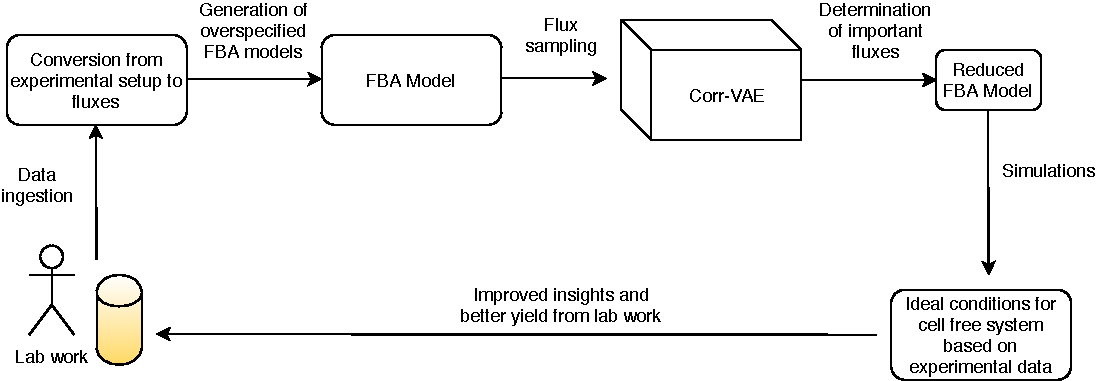
\includegraphics[width=\textwidth]{figs/SystemOverview.pdf}
\end{center}
\label{fig:overview}
\caption{A figure showing the overall pipeline for the system to generate cell-free metabolic models.}
\end{figure}

Chapter \ref{chap:impl} describes the system we have designed and built to model cell-free systems.
The entire pipeline is shown in fig \ref{fig:overview}.
We begin by describing our experimental setup and how we generated our data.
Next, we detail how to ingest the experimental setup and data and convert it into a metabolic model.
Then, we explain how we used that model to generate a larger dataset for our deep learning algorithms.
Lastly, we use that dataset to train a VAE, which generates a lower dimensionality representation that can be used to create better cell-free metabolic models.

Chapter \ref{chap:res} describes the results of the experiments.
This includes results showing the improvement of our system over naive models.
We also show novel biological insights that were unearthed due to my system.
Finally, we illustrate how a model can be learned on one set of biological data and transfer to a different set of data. 

We conclude with a chapter of discussion and directions of future work in this area.
